% !Mode:: "TeX:UTF-8"
\chapter{常见问题}
\label{chapter-faq}
\begin{enumerate}
\item  如何使用visio输出eps图形?
\label{visio2eps}
\begin{itemize}
	\item WindowsXP用户安装Generic PostScript Printer打印机,Windows7用户安装MS Publisher Color Print打印机;
	\item 启动Visio,打开相应的vsd图;
	\item 打开"文件"菜单下的"打印\dots "菜单项,在打印对话框中选择打印机为"Generic PostScriptPrint"或"MS Publisher Color Print";
	\item 点击属性按键,打开属性对话框,再点击高级按键,打开高级选项对话框,纸张规格选择为"Letter";
	\item 在"PostScript选项"的"PostScript输出选项"里选择"内嵌的PostScript(EPS)",然后确定;
	\item 回到打印对话框,在"打印到文件"对话框中输入文件名,扩展名须为.ps(如abc.ps);
	\item 用GSview打开abc.ps,打开"File"菜单里的"PS to EPS"菜单项,按默认的选项(自动计算边框),并在"另存为"对话框中输入最终的eps文件名(如abc.eps)即可。
\end{itemize}
\item 如何将Mathtype的公式转化为\LaTeX{}公式语言?
\label{mathtype2latex}
\begin{itemize}
	\item 安装Mathtype,启动Mathtype;
	\item 转化设置:在菜单Preferences下,选择Translators选项,在弹出的对话框中,
按照如图\ref{fig-fqa-mathtype1}进行设置\footnote{{\heiti 注意}:file下面的两个选项不要选择,
会在转化时会出来很多信息,这些信息对于公式编译没有关系。所以建议不要选,
如若有兴趣的话,可以选中后实验一下。};
\item 在Mathtype中输入公式;
\item 选中公式,复制到\texttt{.tex}的源文件中,编译即可。
\item[{\heiti 注意:}] 使用MathType输入公式然后转化,这样的输入效率比较低,
而且有些LaTeX提供的公式功能,他也无法实现例如:公式的对齐,编号等等,Mathtype适合初学者使用,
建议学习\LaTeX{}公式输入语言。
\end{itemize}
\begin{figure}
\begin{center}
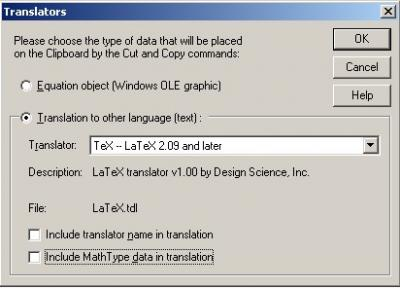
\includegraphics[width=.7\textwidth]{figure/faq-mathtype1.jpg}
\end{center}
\caption{Mathtype中转换设置}\label{fig-fqa-mathtype1}
\end{figure}
\end{enumerate}